% ---------------------------------------------------------
% PySCIPOpt Workshop -- Part 1: Modeling Basics
% Compiles with: pdflatex part1.tex
% ---------------------------------------------------------
\documentclass[aspectratio=169,10pt]{beamer}

\usetheme{Madrid}

% ---- SCIP blue color scheme --------------------------------
\definecolor{scipblue}{RGB}{30,60,190}
\setbeamercolor{structure}{fg=scipblue}
\setbeamercolor{palette primary}{bg=scipblue, fg=white}
\setbeamercolor{palette secondary}{bg=scipblue!85!black, fg=white}
\setbeamercolor{palette tertiary}{bg=scipblue!70!black, fg=white}
\setbeamercolor{palette quaternary}{bg=scipblue, fg=white}
\setbeamercolor{frametitle}{bg=scipblue!10, fg=scipblue}
\setbeamercolor{title}{fg=white, bg=scipblue}
\setbeamercolor{item}{fg=scipblue}

% ---- packages -------------------------------------------
\usepackage{amsmath,amssymb}
\usepackage{tikz}
\usetikzlibrary{arrows.meta,positioning,shapes.geometric,fit}
\usepackage{listings}
\usepackage{booktabs}

% ---- listings style for Python --------------------------
\lstdefinestyle{pyStyle}{
  language=Python,
  basicstyle=\ttfamily\scriptsize,
  keywordstyle=\color{blue!80!black}\bfseries,
  commentstyle=\color{green!50!black}\itshape,
  stringstyle=\color{red!70!black},
  showstringspaces=false,
  breaklines=true,
  frame=single,
  framerule=0.4pt,
  backgroundcolor=\color{gray!5},
  xleftmargin=4pt,
  xrightmargin=4pt,
  aboveskip=6pt,
  belowskip=4pt,
  morekeywords={Model,addVar,addCons,optimize,getVal,getObjVal,
                 getStatus,setMaximize,quicksum,
                 hideOutput,printStatistics},
}
\lstset{style=pyStyle}

% ---- metadata -------------------------------------------
\title{SCIP Workshop}
\subtitle{Part 1: Modeling Basics}
\author{João Dionísio}
\date{March 20th, 2026}
\titlegraphic{%
  
\includegraphics[height=1.2cm]{sciplogo.png}\hspace{1.5cm}%
  
\includegraphics[height=1.2cm]{uporto_logo.jpg}\hspace{1.5cm}%
  
\includegraphics[height=1.2cm]{apdio_logo.png}%
}

% =========================================================
\begin{document}

% ---------------------------------------------------------
% Frame 1: Title
% ---------------------------------------------------------
\begin{frame}
\titlepage
\end{frame}

% ---------------------------------------------------------
% Frame 2: Objectives
% ---------------------------------------------------------
\begin{frame}{Objectives}
By the end of Part~1 you will be able to:
\begin{itemize}
  \item Formulate \textbf{Linear Programs (LP)}, \textbf{Integer Programs (IP)},
        and \textbf{Mixed-Integer Programs (MIP)} in PySCIPOpt.
  \item Translate a mathematical model into Python code.
  \item Solve classical optimization problems:
    \begin{itemize}
      \item Transportation, Portfolio Optimization, Set Cover,
      \item Knapsack, Facility Location, Graph Coloring.
    \end{itemize}
  \item Extract solutions and solver statistics.
\end{itemize}
\end{frame}

% ---------------------------------------------------------
% Frame 3: What is SCIP / PySCIPOpt
% ---------------------------------------------------------
\begin{frame}{What is SCIP / PySCIPOpt?}
\begin{columns}[T]
\begin{column}{0.55\textwidth}
  \textbf{SCIP} --- \emph{Solving Constraint Integer Programs}
  \begin{itemize}
    \item The fastest academic MINLP solver.
    \item Supports LP, MIP, MINLP, CIP.
    \item Open-source (Apache 2.0 license).
    \item Highly extensible plugin architecture.
  \end{itemize}

  \medskip
  \textbf{PySCIPOpt} --- Python interface to SCIP
  \begin{itemize}
    \item Install: \texttt{pip install pyscipopt}
  \end{itemize}
\end{column}
\begin{column}{0.4\textwidth}
  \begin{center}
  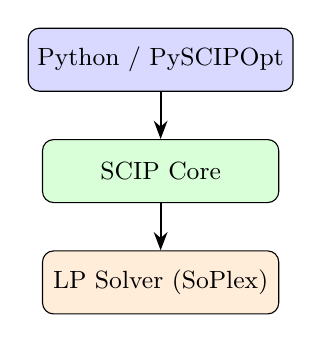
\begin{tikzpicture}[
    box/.style={draw,rounded corners,minimum width=3cm,
                minimum height=0.8cm,align=center,font=\small},
  ]
    \node[box,fill=blue!15]  (py)   {Python / PySCIPOpt};
    \node[box,fill=green!15, below=0.6cm of py]  (scip) {SCIP Core};
    \node[box,fill=orange!15,below=0.6cm of scip](lp)   {LP Solver (SoPlex)};
    \draw[-{Stealth},thick] (py)   -- (scip);
    \draw[-{Stealth},thick] (scip) -- (lp);
  \end{tikzpicture}
  \end{center}
\end{column}
\end{columns}
\end{frame}

% ---------------------------------------------------------
% Frame 4: Model Lifecycle
% ---------------------------------------------------------
\begin{frame}[fragile]{Model Lifecycle}
\begin{center}
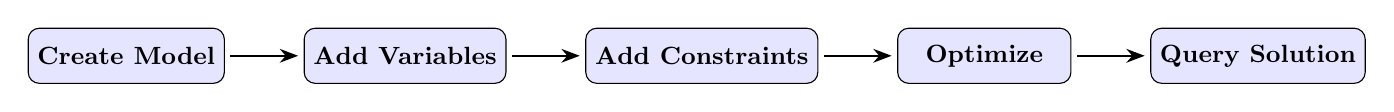
\begin{tikzpicture}[
  stepbox/.style={draw,rounded corners,minimum width=2.2cm,
               minimum height=0.7cm,align=center,font=\small\bfseries,
               fill=blue!10},
  arr/.style={-{Stealth},thick,shorten >=2pt,shorten <=2pt},
]
  \node[stepbox] (create)  {Create Model};
  \node[stepbox,right=1.0cm of create]  (vars)  {Add Variables};
  \node[stepbox,right=1.0cm of vars]    (cons)  {Add Constraints};
  \node[stepbox,right=1.0cm of cons]    (opt)   {Optimize};
  \node[stepbox,right=1.0cm of opt]     (query) {Query Solution};

  \draw[arr] (create) -- (vars);
  \draw[arr] (vars)   -- (cons);
  \draw[arr] (cons)   -- (opt);
  \draw[arr] (opt)    -- (query);
\end{tikzpicture}
\end{center}

\medskip
\begin{lstlisting}
from pyscipopt import Model

model = Model("my_model")     # 1. Create
x = model.addVar(...)         # 2. Variables
model.addCons(...)            # 3. Constraints
model.optimize()              # 4. Optimize
print(model.getVal(x))        # 5. Query
\end{lstlisting}
\end{frame}

% ---------------------------------------------------------
% Frame 5: Variables
% ---------------------------------------------------------
\begin{frame}[fragile]{Variables}
\texttt{model.addVar(name, vtype, lb, ub, obj)}
\medskip
\begin{table}
\centering
\begin{tabular}{lll}
\toprule
\textbf{vtype} & \textbf{Domain} & \textbf{Typical use} \\
\midrule
\texttt{"C"} & Continuous ($\mathbb{R}$) & Quantities, flows \\
\texttt{"B"} & Binary ($\{0,1\}$) & Yes/no decisions \\
\texttt{"I"} & Integer ($\mathbb{Z}$) & Counts \\
\bottomrule
\end{tabular}
\end{table}

\medskip
\begin{lstlisting}
# Binary variable with objective coefficient 3
x = model.addVar(name="x", vtype="B", obj=3)

# Continuous variable in [0, 10]
y = model.addVar(name="y", vtype="C", lb=0, ub=10)

# Integer variable, default bounds [0, +inf)
z = model.addVar(name="z", vtype="I", obj=-2)
\end{lstlisting}
\end{frame}

% ---------------------------------------------------------
% Frame 6: Constraints
% ---------------------------------------------------------
\begin{frame}[fragile]{Constraints}
\texttt{model.addCons(expression, name)}

\begin{lstlisting}

# Single constraint
model.addCons(x + 2*y <= 10, name="capacity")

# Indexed family of constraints
for j in customers:
    model.addCons(
        sum(x[i,j] for i in suppliers) == demand[j],
        name=f"demand_{j}"
    )

model.addCons(sum(c[i]*x[i] for i in I) <= b)
\end{lstlisting}
\end{frame}

% ---------------------------------------------------------
% Frame 7: Objective
% ---------------------------------------------------------
\begin{frame}[fragile]{Objective Function}

\texttt{setObjective}
\begin{lstlisting}
model.setObjective(
    sum(cost[i,j] * x[i,j] for i in I for j in J),
    sense="minimize"
)
\end{lstlisting}

\medskip
Convenience methods:
\begin{itemize}
  \item \texttt{model.setMaximize()} — minimization is the default
\end{itemize}
\end{frame}

% ---------------------------------------------------------
% Frame 8: Exercise 1
% ---------------------------------------------------------
\begin{frame}{Exercise 1: First Model}
\begin{block}{Task}
Build the following model:
\begin{align*}
  \max \quad & 3x + 2y \\
  \text{s.t.} \quad & x + y \le 1 \\
  & 2x + y \le 2 \\
  & x, y \in \{0, 1\}
\end{align*}
\end{block}
\begin{itemize}
  \item File: \texttt{ex01\_first\_model/first\_model.py}
  \item Test: \texttt{python ex01\_first\_model/test\_first\_model.py}
\end{itemize}
\end{frame}

% ---------------------------------------------------------
% Frame 9: Solving
% ---------------------------------------------------------
\begin{frame}[fragile]{Solving and Querying}
\begin{lstlisting}
model.hideOutput()        # suppress solver log (optional)
model.optimize()          # solve the model

status = model.getStatus()    # "optimal", "infeasible", ...
obj    = model.getObjVal()    # objective value
val_x  = model.getVal(x)     # value of variable x
\end{lstlisting}

\medskip
Common status strings:
\begin{table}
\centering\small
\begin{tabular}{ll}
\toprule
\textbf{Status} & \textbf{Meaning} \\
\midrule
\texttt{"optimal"}    & Optimal solution found \\
\texttt{"infeasible"} & No feasible solution exists \\
\texttt{"unbounded"}  & Objective is unbounded \\
\texttt{"timelimit"}  & Time limit reached (may have incumbent) \\
\bottomrule
\end{tabular}
\end{table}
\end{frame}

% ---------------------------------------------------------
% Frame 10: Exercise 2
% ---------------------------------------------------------
\begin{frame}{Exercise 2: Solving}
\begin{block}{Task}
Solve the model from Exercise~1 and extract:
\begin{itemize}
  \item Optimal status, objective value, variable values.
  \item Solver statistics (number of nodes, LP iterations).
\end{itemize}
\end{block}
\begin{itemize}
  \item File: \texttt{ex02\_solving/solving.py}
  \item Test: \texttt{python ex02\_solving/test\_solving.py}
\end{itemize}
\end{frame}

% ---------------------------------------------------------
% Frame 11: Transportation Problem
% ---------------------------------------------------------
\begin{frame}{Transportation Problem}
\begin{columns}[T]
\begin{column}{0.45\textwidth}
\begin{center}
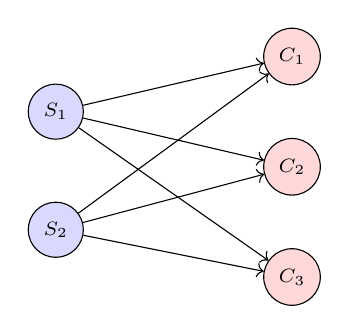
\begin{tikzpicture}[
  sup/.style={circle,draw,fill=blue!15,minimum size=0.7cm,
              font=\scriptsize\bfseries},
  cus/.style={circle,draw,fill=red!15,minimum size=0.7cm,
              font=\scriptsize\bfseries},
  every edge/.style={draw,-{Stealth},thin},
]
  \node[sup] (s1) at (0, 1.5) {$S_1$};
  \node[sup] (s2) at (0, 0)   {$S_2$};
  \node[cus] (c1) at (3, 2.2) {$C_1$};
  \node[cus] (c2) at (3, 0.8) {$C_2$};
  \node[cus] (c3) at (3,-0.6) {$C_3$};

  \foreach \s in {s1,s2}
    \foreach \c in {c1,c2,c3}
      \draw[->] (\s) -- (\c);
\end{tikzpicture}
\end{center}
\end{column}
\begin{column}{0.55\textwidth}
\textbf{Sets:} suppliers $I$, customers $J$

\textbf{Parameters:} supply $s_i$, demand $d_j$, cost $c_{ij}$

\textbf{Variables:} $x_{ij} \ge 0$ (flow from $i$ to $j$)

\begin{align*}
  \min \quad & \sum_{i \in I}\sum_{j \in J} c_{ij}\, x_{ij} \\
  \text{s.t.} \quad
    & \sum_{j \in J} x_{ij} \le s_i  & \forall\, i \in I \\
    & \sum_{i \in I} x_{ij} \ge d_j  & \forall\, j \in J \\
    & x_{ij} \ge 0
\end{align*}
\end{column}
\end{columns}
\end{frame}

% ---------------------------------------------------------
% Frame 12: Data in Python
% ---------------------------------------------------------
\begin{frame}[fragile]{Data in Python --- Dictionaries and Loops}
\begin{lstlisting}
# Data as dictionaries
supply   = {"S1": 100, "S2": 150}
demand   = {"C1": 80, "C2": 90, "C3": 70}
cost     = {("S1","C1"): 4, ("S1","C2"): 6, ("S1","C3"): 9,
            ("S2","C1"): 5, ("S2","C2"): 3, ("S2","C3"): 7}

# Variables via nested comprehension
x = {(i,j): model.addVar(name=f"x_{i}_{j}", vtype="C")
     for i in supply for j in demand}

# Constraints via loops
for i in supply:
    model.addCons(
        quicksum(x[i,j] for j in demand) <= supply[i])
for j in demand:
    model.addCons(
        quicksum(x[i,j] for i in supply) >= demand[j])
\end{lstlisting}
\end{frame}

% ---------------------------------------------------------
% Frame 13: Exercise 3
% ---------------------------------------------------------
\begin{frame}{Exercise 3: Transportation}
\begin{block}{Task}
Implement the transportation problem:
\begin{itemize}
  \item Read data from provided dictionaries.
  \item Build variables, supply/demand constraints, minimize cost.
  \item Print optimal shipment plan.
\end{itemize}
\end{block}
\begin{itemize}
  \item File: \texttt{ex03\_transportation/transportation.py}
  \item Test: \texttt{python ex03\_transportation/test\_transportation.py}
\end{itemize}
\end{frame}

% ---------------------------------------------------------
% Frame 14: Portfolio Optimization
% ---------------------------------------------------------
\begin{frame}{Portfolio Optimization (Markowitz)}
\begin{columns}[T]
\begin{column}{0.42\textwidth}
\begin{center}
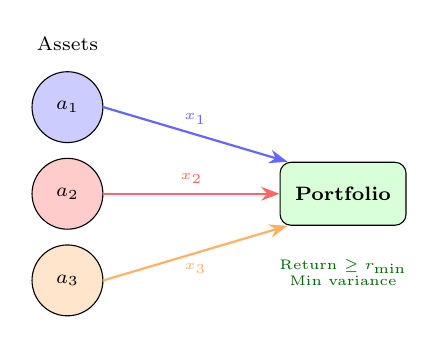
\begin{tikzpicture}[
  asset/.style={circle,draw,minimum size=0.9cm,
                font=\scriptsize\bfseries},
  port/.style={rectangle,draw,rounded corners=4pt,fill=green!15,
               minimum width=1.6cm,minimum height=0.8cm,
               font=\scriptsize\bfseries},
  arr/.style={-{Stealth},thick},
]
  % Assets
  \node[asset,fill=blue!20]   (a1) at (0, 1.6) {$a_1$};
  \node[asset,fill=red!20]    (a2) at (0, 0.5) {$a_2$};
  \node[asset,fill=orange!20] (a3) at (0,-0.6) {$a_3$};

  \node[anchor=south,font=\scriptsize] at (0,2.2) {Assets};

  % Portfolio
  \node[port] (p) at (3.5,0.5) {Portfolio};

  % Arrows with weights
  \draw[arr,blue!60]   (a1.east) -- node[above,font=\tiny]{$x_1$} (p.150);
  \draw[arr,red!60]    (a2.east) -- node[above,font=\tiny]{$x_2$} (p.west);
  \draw[arr,orange!60] (a3.east) -- node[below,font=\tiny]{$x_3$} (p.210);

  % Annotations
  \node[below=0.3cm of p,font=\tiny,align=center,text=green!40!black]
    {Return $\ge r_{\min}$\\Min variance};
\end{tikzpicture}
\end{center}
\end{column}
\begin{column}{0.58\textwidth}
Allocate capital among assets to minimize risk (variance) while achieving a target return.

\smallskip
{\small\textbf{Parameters:} returns $\mu_i$, covariance $\Sigma_{ij}$, target $r_{\min}$}

{\small\textbf{Variables:} $x_i \in [0,1]$ (weight of asset $i$)}

\begin{align*}
  \min \quad & t \\
  \text{s.t.} \quad
    & t \ge \textstyle\sum_{i}\sum_{j} \Sigma_{ij}\, x_i \, x_j \\
    & \sum_i \mu_i\, x_i \ge r_{\min} \\
    & \sum_i x_i = 1, \quad 0 \le x_i \le 1
\end{align*}

\smallskip
{\small\textbf{Note:} SCIP needs a linear objective, so we use the epigraph trick: minimize $t$ subject to $t \ge x^\top\!\Sigma\, x$.}
\end{column}
\end{columns}
\end{frame}

% ---------------------------------------------------------
% Frame 15: Exercise 4
% ---------------------------------------------------------
\begin{frame}{Exercise 4: Portfolio Optimization}
\begin{block}{Task}
Implement the Markowitz portfolio model:
\begin{itemize}
  \item Budget and return constraints (linear).
  \item Auxiliary variable $t$ with \texttt{obj=1}.
  \item \textbf{Quadratic constraint}: $t \ge x^\top \Sigma\, x$.
\end{itemize}
\end{block}
\begin{itemize}
  \item File: \texttt{ex04\_portfolio/portfolio.py}
  \item Test: \texttt{python ex04\_portfolio/test\_portfolio.py}
\end{itemize}
\end{frame}

% ---------------------------------------------------------
% Frame 16: Set Cover
% ---------------------------------------------------------
\begin{frame}{From LP to IP: Set Cover}
\begin{columns}[T]
\begin{column}{0.42\textwidth}
\begin{center}
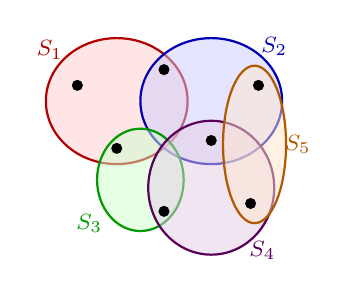
\begin{tikzpicture}
  % --- Sets (ellipses drawn first, elements on top) ---
  % S1 = elements {a,b,d}
  \fill[red!20, fill opacity=0.5] (0.7, 1.8) ellipse (0.9 and 0.8);
  \draw[red!70!black, thick] (0.7, 1.8) ellipse (0.9 and 0.8);
  % S2 = elements {b,c,e}
  \fill[blue!20, fill opacity=0.5] (1.9, 1.8) ellipse (0.9 and 0.8);
  \draw[blue!70!black, thick] (1.9, 1.8) ellipse (0.9 and 0.8);
  % S3 = elements {d,f}
  \fill[green!20, fill opacity=0.5] (1.0, 0.8) ellipse (0.55 and 0.65);
  \draw[green!60!black, thick] (1.0, 0.8) ellipse (0.55 and 0.65);
  % S4 = elements {e,f,g}
  \fill[violet!20, fill opacity=0.5] (1.9, 0.7) ellipse (0.8 and 0.85);
  \draw[violet!70!black, thick] (1.9, 0.7) ellipse (0.8 and 0.85);
  % S5 = elements {c,g}
  \fill[orange!20, fill opacity=0.5] (2.45, 1.25) ellipse (0.4 and 1.0);
  \draw[orange!70!black, thick] (2.45, 1.25) ellipse (0.4 and 1.0);

  % --- Set labels (outside their ellipses) ---
  \node[font=\footnotesize\bfseries, red!70!black] at (-0.15, 2.45) {$S_1$};
  \node[font=\footnotesize\bfseries, blue!70!black] at (2.7, 2.5) {$S_2$};
  \node[font=\footnotesize\bfseries, green!60!black] at (0.35, 0.25) {$S_3$};
  \node[font=\footnotesize\bfseries, violet!70!black] at (2.55, -0.1) {$S_4$};
  \node[font=\footnotesize\bfseries, orange!70!black] at (3.0, 1.25) {$S_5$};

  % --- Universe elements (dots) ---
  \foreach \pos in {(0.2,2.0), (1.3,2.2), (2.5,2.0),
                    (0.7,1.2), (1.9,1.3),
                    (1.3,0.4), (2.4,0.5)}
    \fill[black] \pos circle (2pt);
\end{tikzpicture}
\end{center}
\vspace{-2pt}
{\centering\scriptsize Select cheapest combination of sets to cover all elements.\par}
\end{column}
\begin{column}{0.58\textwidth}
\textbf{Given:} Universe $U = \{1,\dots,n\}$, subsets $S_1,\dots,S_m \subseteq U$,
costs $c_j$.

\textbf{Goal:} Select minimum-cost subsets that cover every element.

\smallskip
\textbf{Variables:} $x_j \in \{0,1\}$ (select subset $j$?)

\begin{align*}
  \min \quad & \sum_{j=1}^{m} c_j \, x_j \\
  \text{s.t.} \quad
    & \sum_{j:\, i \in S_j} x_j \ge 1
      & \forall\, i \in U \\
    & x_j \in \{0,1\}
      & \forall\, j
\end{align*}

\smallskip
\begin{itemize}
  \item This is a \textbf{pure integer program} (all variables binary).
  \item LP relaxation gives a lower bound; SCIP uses branch-and-bound.
\end{itemize}
\end{column}
\end{columns}
\end{frame}

% ---------------------------------------------------------
% Frame 17: Exercise 5
% ---------------------------------------------------------
\begin{frame}{Exercise 5: Set Cover}
\begin{block}{Task}
Implement the set cover problem:
\begin{itemize}
  \item Define binary variables for each subset.
  \item Add covering constraints for each element.
  \item Minimize total cost.
\end{itemize}
\end{block}
\begin{itemize}
  \item File: \texttt{ex05\_set\_cover/set\_cover.py}
  \item Test: \texttt{python ex05\_set\_cover/test\_set\_cover.py}
\end{itemize}
\end{frame}

% ---------------------------------------------------------
% Frame 18: Knapsack Problem
% ---------------------------------------------------------
\begin{frame}{Knapsack Problem}
\begin{columns}[T]
\begin{column}{0.43\textwidth}
\begin{center}
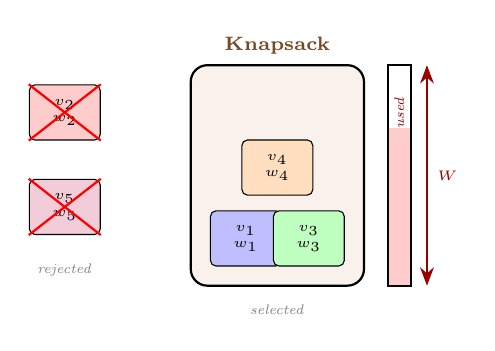
\begin{tikzpicture}[
  item/.style={rectangle,draw,rounded corners=2pt,minimum width=0.9cm,
               minimum height=0.7cm,font=\tiny,align=center},
  arr/.style={-{Stealth},thick,dashed,gray},
]
  % Knapsack (bag)
  \draw[thick,fill=brown!10,rounded corners=6pt]
    (2.0,-0.2) rectangle (4.2,2.6);
  \node[font=\scriptsize\bfseries,brown!60!black] at (3.1,2.85) {Knapsack};

  % Capacity bar
  \draw[thick,gray] (4.5,-0.2) -- (4.5,2.6);
  \fill[red!20] (4.5,-0.2) rectangle (4.8,1.8);
  \draw[thick] (4.5,-0.2) rectangle (4.8,2.6);
  \draw[thick,red!60!black,{Stealth}-{Stealth}] (5.0,-0.2) -- node[right,font=\tiny]{$W$} (5.0,2.6);
  \node[font=\tiny,red!60!black] at (4.65,2.0) {\rotatebox{90}{\textit{used}}};

  % Items inside bag (selected)
  \node[item,fill=blue!25]   at (2.7,0.4) {$v_1$\\$w_1$};
  \node[item,fill=green!25]  at (3.5,0.4) {$v_3$\\$w_3$};
  \node[item,fill=orange!25] at (3.1,1.3) {$v_4$\\$w_4$};

  % Items outside (not selected)
  \node[item,fill=red!20]    (out1) at (0.4,2.0) {$v_2$\\$w_2$};
  \node[item,fill=purple!20] (out2) at (0.4,0.8) {$v_5$\\$w_5$};

  % Cross marks on excluded items
  \draw[red,thick] (out1.north west) -- (out1.south east);
  \draw[red,thick] (out1.south west) -- (out1.north east);
  \draw[red,thick] (out2.north west) -- (out2.south east);
  \draw[red,thick] (out2.south west) -- (out2.north east);

  % Labels
  \node[font=\tiny,gray] at (0.4,0.0) {\textit{rejected}};
  \node[font=\tiny,gray] at (3.1,-0.5) {\textit{selected}};
\end{tikzpicture}
\end{center}
\end{column}
\begin{column}{0.57\textwidth}
\textbf{Classic 0--1 Knapsack:} select items to maximize value
without exceeding capacity.

\smallskip
{\small\textbf{Applications:} budgeting, cargo loading, resource allocation.}

\smallskip
\textbf{Variables:} $x_j \in \{0,1\}$ (take item $j$?)

\begin{align*}
  \max \quad & \sum_{j=1}^{n} v_j \, x_j \\
  \text{s.t.} \quad
    & \sum_{j=1}^{n} w_j \, x_j \le W \\
    & x_j \in \{0,1\} & \forall\, j
\end{align*}

{\small where $v_j$ = value, $w_j$ = weight, $W$ = capacity.}

\end{column}
\end{columns}
\end{frame}

% ---------------------------------------------------------
% Frame 19: Exercise 6
% ---------------------------------------------------------
\begin{frame}{Exercise 6: Knapsack}
\begin{block}{Task}
Implement the 0--1 knapsack problem:
\begin{itemize}
  \item Create binary variables for each item.
  \item Add the capacity constraint.
  \item Maximize total value and report selected items.
\end{itemize}
\end{block}
\begin{itemize}
  \item File: \texttt{ex06\_knapsack/knapsack.py}
  \item Test: \texttt{python ex06\_knapsack/test\_knapsack.py}
\end{itemize}
\end{frame}

% ---------------------------------------------------------
% Frame 20: Facility Location
% ---------------------------------------------------------
\begin{frame}{Facility Location}
\begin{columns}[T]
\begin{column}{0.40\textwidth}
\begin{center}
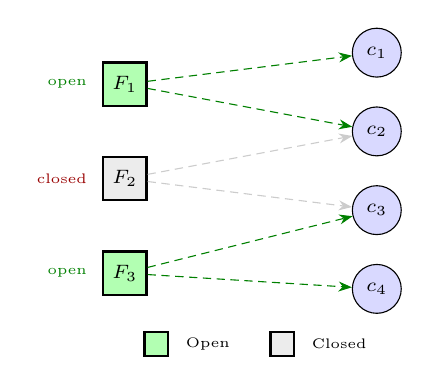
\begin{tikzpicture}[
  fac/.style={rectangle,draw,minimum size=0.55cm,font=\scriptsize\bfseries,
              thick},
  cust/.style={circle,draw,fill=blue!15,minimum size=0.5cm,
               font=\scriptsize\bfseries},
  assign/.style={-{Stealth},thin,densely dashed},
]
  % Facilities (left column)
  \node[fac,fill=green!30]  (f1) at (0, 2.2) {$F_1$};
  \node[fac,fill=gray!15]   (f2) at (0, 1.0) {$F_2$};
  \node[fac,fill=green!30]  (f3) at (0,-0.2) {$F_3$};

  % Open/closed labels
  \node[font=\tiny,green!50!black,left=2pt of f1] {open};
  \node[font=\tiny,red!60!black,left=2pt of f2] {closed};
  \node[font=\tiny,green!50!black,left=2pt of f3] {open};

  % Customers (right column)
  \node[cust] (c1) at (3.2, 2.6) {$c_1$};
  \node[cust] (c2) at (3.2, 1.6) {$c_2$};
  \node[cust] (c3) at (3.2, 0.6) {$c_3$};
  \node[cust] (c4) at (3.2,-0.4) {$c_4$};

  % Assignment edges (from open facilities only)
  \draw[assign,green!50!black] (f1) -- (c1);
  \draw[assign,green!50!black] (f1) -- (c2);
  \draw[assign,green!50!black] (f3) -- (c3);
  \draw[assign,green!50!black] (f3) -- (c4);

  % Grey dashed from closed facility (potential)
  \draw[assign,gray!40] (f2) -- (c2);
  \draw[assign,gray!40] (f2) -- (c3);

  % Legend
  \node[fac,fill=green!30,minimum size=0.3cm] at (0.4,-1.1) {};
  \node[font=\tiny,right] at (0.65,-1.1) {Open};
  \node[fac,fill=gray!15,minimum size=0.3cm] at (2.0,-1.1) {};
  \node[font=\tiny,right] at (2.25,-1.1) {Closed};
\end{tikzpicture}
\end{center}
\end{column}
\begin{column}{0.60\textwidth}
\textbf{Decide} which facilities to open and how to assign customers.

\smallskip
{\small\textbf{Sets:} facilities $F$, customers $C$}

{\small\textbf{Parameters:} fixed cost $f_i$, assignment cost $t_{ij}$, demand $d_j$, capacity $q_i$}

{\small\textbf{Variables:} $y_i \in \{0,1\}$ (open $i$?), \; $x_{ij} \ge 0$ (fraction served)}

\begin{align*}
  \min \quad & \sum_{i \in F} f_i\, y_i
    + \sum_{i \in F}\sum_{j \in C} t_{ij}\, x_{ij} \\
  \text{s.t.} \quad
    & \sum_{i \in F} x_{ij} = 1
      & \forall\, j \in C \\
    & \sum_{j \in C} d_j\, x_{ij} \le q_i\, y_i
      & \forall\, i \in F \\
    & x_{ij} \ge 0,\; y_i \in \{0,1\}
\end{align*}

\begin{itemize}
  \item The constraint $x_{ij} \le y_i$ \textbf{links} assignment to opening.
\end{itemize}
\end{column}
\end{columns}
\end{frame}

% ---------------------------------------------------------
% Frame 21: Exercise 7
% ---------------------------------------------------------
\begin{frame}{Exercise 7: Facility Location}
\begin{block}{Task}
Implement the uncapacitated facility location problem:
\begin{itemize}
  \item Binary variables for facility opening decisions.
  \item Continuous variables for customer assignments.
  \item Linking and demand constraints.
\end{itemize}
\end{block}
\begin{itemize}
  \item File: \texttt{ex07\_facility\_location/facility\_location.py}
  \item Test: \texttt{python ex07\_facility\_location/test\_facility\_location.py}
\end{itemize}
\end{frame}

% ---------------------------------------------------------
% Frame 22: Graph Coloring
% ---------------------------------------------------------
\begin{frame}{Graph Coloring}
\begin{columns}[T]
\begin{column}{0.40\textwidth}
\begin{center}
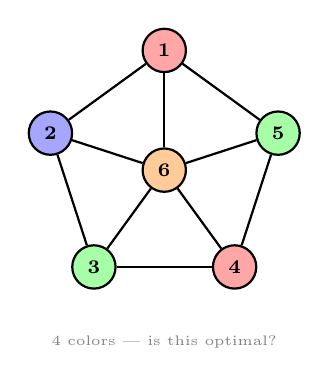
\begin{tikzpicture}[
  vtx/.style={circle,draw,thick,minimum size=0.55cm,font=\scriptsize\bfseries,
              inner sep=0pt},
  edge/.style={thick},
  scale=0.95,
]
  % Pentagon vertices
  \node[vtx,fill=red!35]    (v1) at (90:1.6)  {1};
  \node[vtx,fill=blue!35]   (v2) at (162:1.6) {2};
  \node[vtx,fill=green!35]  (v3) at (234:1.6) {3};
  \node[vtx,fill=red!35]    (v4) at (306:1.6) {4};
  \node[vtx,fill=green!35]  (v5) at (18:1.6)  {5};

  % Inner star vertex (center)
  \node[vtx,fill=orange!40] (v6) at (0,0) {6};

  % Outer edges (pentagon)
  \draw[edge] (v1) -- (v2);
  \draw[edge] (v2) -- (v3);
  \draw[edge] (v3) -- (v4);
  \draw[edge] (v4) -- (v5);
  \draw[edge] (v5) -- (v1);

  % Inner edges (star from center)
  \draw[edge] (v6) -- (v1);
  \draw[edge] (v6) -- (v2);
  \draw[edge] (v6) -- (v3);
  \draw[edge] (v6) -- (v4);
  \draw[edge] (v6) -- (v5);

  % Color legend
  \node[font=\tiny,gray] at (0,-2.3) {4 colors --- is this optimal?};
\end{tikzpicture}
\end{center}
\end{column}
\begin{column}{0.60\textwidth}
\textbf{Given:} undirected graph $G=(V,E)$, set of colors $K=\{1,\dots,k\}$.

\textbf{Goal:} minimize the number of colors used such that
no two adjacent vertices share a color.

\smallskip
{\small\textbf{Variables:} $x_{v,c} \in \{0,1\}$ (vertex $v$ gets color $c$?), \;
$w_c \in \{0,1\}$ (color $c$ used?)}

\begin{align*}
  \min \quad & \sum_{c \in K} w_c \\
  \text{s.t.} \quad
    & \sum_{c \in K} x_{v,c} = 1
      & \forall\, v \in V \\
    & x_{u,c} + x_{v,c} \le w_c
      & \forall\, (u,v) \in E,\; c \in K \\
    & x_{v,c},\, w_c \in \{0,1\}
\end{align*}

{\small
\textbf{Symmetry:} permuting colors $\Rightarrow$ equivalent solution.\\
\textbf{Break:} $w_1 \ge w_2 \ge \cdots \ge w_k$.}
\end{column}
\end{columns}
\end{frame}

% ---------------------------------------------------------
% Frame 23: Exercise 8
% ---------------------------------------------------------
\begin{frame}{Exercise 8: Graph Coloring}
\begin{block}{Task}
Implement the graph coloring formulation:
\begin{itemize}
  \item Assignment and conflict constraints.
  \item Minimize number of colors.
  \item Add symmetry-breaking constraints.
\end{itemize}
\end{block}
\begin{itemize}
  \item File: \texttt{ex08\_graph\_coloring/graph\_coloring.py}
  \item Test: \texttt{python ex08\_graph\_coloring/test\_graph\_coloring.py}
\end{itemize}
\end{frame}

% ---------------------------------------------------------
% Frame 24: Wrap-up
% ---------------------------------------------------------
\begin{frame}{Part 1 --- Wrap-up}
\textbf{What we covered:}
\begin{itemize}
  \item The PySCIPOpt modeling lifecycle: variables, constraints, objective.
  \item Solving and querying solutions and statistics.
  \item Classical LP/IP/MIP formulations:
    \begin{itemize}
      \item Transportation (LP)
      \item Portfolio Optimization (QP)
      \item Set Cover (IP)
      \item Knapsack (IP)
      \item Facility Location (MIP)
      \item Graph Coloring (IP)
    \end{itemize}
\end{itemize}

\medskip
\begin{block}{Up next --- Part 2: Advanced Topics}
\begin{itemize}
  \item Row generation (cutting planes, lazy constraints)
  \item Column generation
  \item Branch-and-Price
\end{itemize}
\end{block}
\end{frame}

\end{document}
